\documentclass[1p]{elsarticle_modified}
%\bibliographystyle{elsarticle-num}

%\usepackage[colorlinks]{hyperref}
%\usepackage{abbrmath_seonhwa} %\Abb, \Ascr, \Acal ,\Abf, \Afrak
\usepackage{amsfonts}
\usepackage{amssymb}
\usepackage{amsmath}
\usepackage{amsthm}
\usepackage{scalefnt}
\usepackage{amsbsy}
\usepackage{kotex}
\usepackage{caption}
\usepackage{subfig}
\usepackage{color}
\usepackage{graphicx}
\usepackage{xcolor} %% white, black, red, green, blue, cyan, magenta, yellow
\usepackage{float}
\usepackage{setspace}
\usepackage{hyperref}

\usepackage{tikz}
\usetikzlibrary{arrows}

\usepackage{multirow}
\usepackage{array} % fixed length table
\usepackage{hhline}

%%%%%%%%%%%%%%%%%%%%%
\makeatletter
\renewcommand*\env@matrix[1][\arraystretch]{%
	\edef\arraystretch{#1}%
	\hskip -\arraycolsep
	\let\@ifnextchar\new@ifnextchar
	\array{*\c@MaxMatrixCols c}}
\makeatother %https://tex.stackexchange.com/questions/14071/how-can-i-increase-the-line-spacing-in-a-matrix
%%%%%%%%%%%%%%%

\usepackage[normalem]{ulem}

\newcommand{\msout}[1]{\ifmmode\text{\sout{\ensuremath{#1}}}\else\sout{#1}\fi}
%SOURCE: \msout is \stkout macro in https://tex.stackexchange.com/questions/20609/strikeout-in-math-mode

\newcommand{\cancel}[1]{
	\ifmmode
	{\color{red}\msout{#1}}
	\else
	{\color{red}\sout{#1}}
	\fi
}

\newcommand{\add}[1]{
	{\color{blue}\uwave{#1}}
}

\newcommand{\replace}[2]{
	\ifmmode
	{\color{red}\msout{#1}}{\color{blue}\uwave{#2}}
	\else
	{\color{red}\sout{#1}}{\color{blue}\uwave{#2}}
	\fi
}

\newcommand{\Sol}{\mathcal{S}} %segment
\newcommand{\D}{D} %diagram
\newcommand{\A}{\mathcal{A}} %arc


%%%%%%%%%%%%%%%%%%%%%%%%%%%%%5 test

\def\sl{\operatorname{\textup{SL}}(2,\Cbb)}
\def\psl{\operatorname{\textup{PSL}}(2,\Cbb)}
\def\quan{\mkern 1mu \triangleright \mkern 1mu}

\theoremstyle{definition}
\newtheorem{thm}{Theorem}[section]
\newtheorem{prop}[thm]{Proposition}
\newtheorem{lem}[thm]{Lemma}
\newtheorem{ques}[thm]{Question}
\newtheorem{cor}[thm]{Corollary}
\newtheorem{defn}[thm]{Definition}
\newtheorem{exam}[thm]{Example}
\newtheorem{rmk}[thm]{Remark}
\newtheorem{alg}[thm]{Algorithm}

\newcommand{\I}{\sqrt{-1}}
\begin{document}

%\begin{frontmatter}
%
%\title{Boundary parabolic representations of knots up to 8 crossings}
%
%%% Group authors per affiliation:
%\author{Yunhi Cho} 
%\address{Department of Mathematics, University of Seoul, Seoul, Korea}
%\ead{yhcho@uos.ac.kr}
%
%
%\author{Seonhwa Kim} %\fnref{s_kim}}
%\address{Center for Geometry and Physics, Institute for Basic Science, Pohang, 37673, Korea}
%\ead{ryeona17@ibs.re.kr}
%
%\author{Hyuk Kim}
%\address{Department of Mathematical Sciences, Seoul National University, Seoul 08826, Korea}
%\ead{hyukkim@snu.ac.kr}
%
%\author{Seokbeom Yoon}
%\address{Department of Mathematical Sciences, Seoul National University, Seoul, 08826,  Korea}
%\ead{sbyoon15@snu.ac.kr}
%
%\begin{abstract}
%We find all boundary parabolic representation of knots up to 8 crossings.
%
%\end{abstract}
%\begin{keyword}
%    \MSC[2010] 57M25 
%\end{keyword}
%
%\end{frontmatter}

%\linenumbers
%\tableofcontents
%
\newcommand\colored[1]{\textcolor{white}{\rule[-0.35ex]{0.8em}{1.4ex}}\kern-0.8em\color{red} #1}%
%\newcommand\colored[1]{\textcolor{white}{ #1}\kern-2.17ex	\textcolor{white}{ #1}\kern-1.81ex	\textcolor{white}{ #1}\kern-2.15ex\color{red}#1	}

{\Large $\underline{12a_{1153}~(K12a_{1153})}$}

\setlength{\tabcolsep}{10pt}
\renewcommand{\arraystretch}{1.6}
\vspace{1cm}\begin{tabular}{m{100pt}>{\centering\arraybackslash}m{274pt}}
\multirow{5}{120pt}{
	\centering
	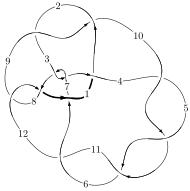
\includegraphics[width=112pt]{../../../GIT/diagram.site/Diagrams/png/1954_12a_1153.png}\\
\ \ \ A knot diagram\footnotemark}&
\allowdisplaybreaks
\textbf{Linearized knot diagam} \\
\cline{2-2}
 &
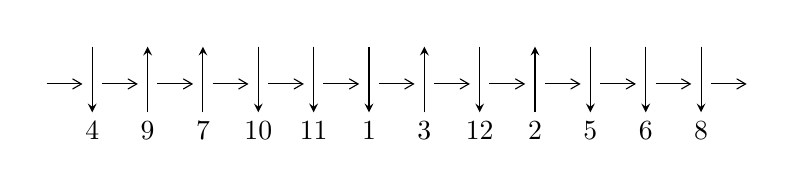
\begin{tikzpicture}[x=20pt, y=17pt]
	% nodes
	\node (C0) at (0, 0) {};
	\node (C1) at (1, 0) {};
	\node (C1U) at (1, +1) {};
	\node (C1D) at (1, -1) {4};

	\node (C2) at (2, 0) {};
	\node (C2U) at (2, +1) {};
	\node (C2D) at (2, -1) {9};

	\node (C3) at (3, 0) {};
	\node (C3U) at (3, +1) {};
	\node (C3D) at (3, -1) {7};

	\node (C4) at (4, 0) {};
	\node (C4U) at (4, +1) {};
	\node (C4D) at (4, -1) {10};

	\node (C5) at (5, 0) {};
	\node (C5U) at (5, +1) {};
	\node (C5D) at (5, -1) {11};

	\node (C6) at (6, 0) {};
	\node (C6U) at (6, +1) {};
	\node (C6D) at (6, -1) {1};

	\node (C7) at (7, 0) {};
	\node (C7U) at (7, +1) {};
	\node (C7D) at (7, -1) {3};

	\node (C8) at (8, 0) {};
	\node (C8U) at (8, +1) {};
	\node (C8D) at (8, -1) {12};

	\node (C9) at (9, 0) {};
	\node (C9U) at (9, +1) {};
	\node (C9D) at (9, -1) {2};

	\node (C10) at (10, 0) {};
	\node (C10U) at (10, +1) {};
	\node (C10D) at (10, -1) {5};

	\node (C11) at (11, 0) {};
	\node (C11U) at (11, +1) {};
	\node (C11D) at (11, -1) {6};

	\node (C12) at (12, 0) {};
	\node (C12U) at (12, +1) {};
	\node (C12D) at (12, -1) {8};
	\node (C13) at (13, 0) {};

	% arrows
	\draw[->,>={angle 60}]
	(C0) edge (C1) (C1) edge (C2) (C2) edge (C3) (C3) edge (C4) (C4) edge (C5) (C5) edge (C6) (C6) edge (C7) (C7) edge (C8) (C8) edge (C9) (C9) edge (C10) (C10) edge (C11) (C11) edge (C12) (C12) edge (C13) ;	\draw[->,>=stealth]
	(C1U) edge (C1D) (C2D) edge (C2U) (C3D) edge (C3U) (C4U) edge (C4D) (C5U) edge (C5D) (C6U) edge (C6D) (C7D) edge (C7U) (C8U) edge (C8D) (C9D) edge (C9U) (C10U) edge (C10D) (C11U) edge (C11D) (C12U) edge (C12D) ;
	\end{tikzpicture} \\
\hhline{~~} \\& 
\textbf{Solving Sequence} \\ \cline{2-2} 
 &
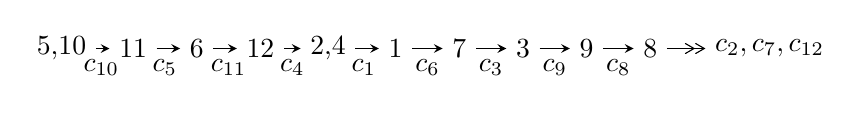
\begin{tikzpicture}[x=23pt, y=7pt]
	% node
	\node (A0) at (-1/8, 0) {5,10};
	\node (A1) at (1, 0) {11};
	\node (A2) at (2, 0) {6};
	\node (A3) at (3, 0) {12};
	\node (A4) at (65/16, 0) {2,4};
	\node (A5) at (41/8, 0) {1};
	\node (A6) at (49/8, 0) {7};
	\node (A7) at (57/8, 0) {3};
	\node (A8) at (65/8, 0) {9};
	\node (A9) at (73/8, 0) {8};
	\node (C1) at (1/2, -1) {$c_{10}$};
	\node (C2) at (3/2, -1) {$c_{5}$};
	\node (C3) at (5/2, -1) {$c_{11}$};
	\node (C4) at (7/2, -1) {$c_{4}$};
	\node (C5) at (37/8, -1) {$c_{1}$};
	\node (C6) at (45/8, -1) {$c_{6}$};
	\node (C7) at (53/8, -1) {$c_{3}$};
	\node (C8) at (61/8, -1) {$c_{9}$};
	\node (C9) at (69/8, -1) {$c_{8}$};
	\node (A10) at (11, 0) {$c_{2},c_{7},c_{12}$};

	% edge
	\draw[->,>=stealth]	
	(A0) edge (A1) (A1) edge (A2) (A2) edge (A3) (A3) edge (A4) (A4) edge (A5) (A5) edge (A6) (A6) edge (A7) (A7) edge (A8) (A8) edge (A9) ;
	\draw[->>,>={angle 60}]	
	(A9) edge (A10);
\end{tikzpicture} \\ 

\end{tabular} \\

\footnotetext{
The image of knot diagram is generated by the software ``\textbf{Draw programme}" developed by Andrew Bartholomew(\url{http://www.layer8.co.uk/maths/draw/index.htm\#Running-draw}), where we modified some parts for our purpose(\url{https://github.com/CATsTAILs/LinksPainter}).
}\phantom \\ \newline 
\centering \textbf{Ideals for irreducible components\footnotemark of $X_{\text{par}}$} 
 
\begin{align*}
I^u_{1}&=\langle 
7.92523\times10^{127} u^{89}+3.07371\times10^{128} u^{88}+\cdots+5.59035\times10^{128} b+1.35846\times10^{130},\\
\phantom{I^u_{1}}&\phantom{= \langle  }-2.38182\times10^{128} u^{89}+6.32318\times10^{129} u^{88}+\cdots+6.42890\times10^{129} a+1.54116\times10^{131},\\
\phantom{I^u_{1}}&\phantom{= \langle  }u^{90}- u^{89}+\cdots+42 u-23\rangle \\
I^u_{2}&=\langle 
u^{19}- u^{18}+\cdots+b- u,\;- u^{19}+u^{18}+\cdots+a- u,\;u^{20}-2 u^{19}+\cdots-7 u^2+1\rangle \\
I^u_{3}&=\langle 
2 b- a-1,\;a^2+3,\;u+1\rangle \\
\\
\end{align*}
\raggedright * 3 irreducible components of $\dim_{\mathbb{C}}=0$, with total 112 representations.\\
\footnotetext{All coefficients of polynomials are rational numbers. But the coefficients are sometimes approximated in decimal forms when there is not enough margin.}
\newpage
\renewcommand{\arraystretch}{1}
\centering \section*{I. $I^u_{1}= \langle 7.93\times10^{127} u^{89}+3.07\times10^{128} u^{88}+\cdots+5.59\times10^{128} b+1.36\times10^{130},\;-2.38\times10^{128} u^{89}+6.32\times10^{129} u^{88}+\cdots+6.43\times10^{129} a+1.54\times10^{131},\;u^{90}- u^{89}+\cdots+42 u-23 \rangle$}
\flushleft \textbf{(i) Arc colorings}\\
\begin{tabular}{m{7pt} m{180pt} m{7pt} m{180pt} }
\flushright $a_{5}=$&$\begin{pmatrix}0\\u\end{pmatrix}$ \\
\flushright $a_{10}=$&$\begin{pmatrix}1\\0\end{pmatrix}$ \\
\flushright $a_{11}=$&$\begin{pmatrix}1\\u^2\end{pmatrix}$ \\
\flushright $a_{6}=$&$\begin{pmatrix}- u\\- u^3+u\end{pmatrix}$ \\
\flushright $a_{12}=$&$\begin{pmatrix}- u^2+1\\- u^4+2 u^2\end{pmatrix}$ \\
\flushright $a_{2}=$&$\begin{pmatrix}0.0370486 u^{89}-0.983555 u^{88}+\cdots+46.7107 u-23.9724\\-0.141766 u^{89}-0.549825 u^{88}+\cdots+26.6619 u-24.3001\end{pmatrix}$ \\
\flushright $a_{4}=$&$\begin{pmatrix}u\\u\end{pmatrix}$ \\
\flushright $a_{1}=$&$\begin{pmatrix}0.154839 u^{89}-0.652648 u^{88}+\cdots+31.8915 u-18.1094\\-0.0239759 u^{89}-0.218917 u^{88}+\cdots+11.8427 u-18.4371\end{pmatrix}$ \\
\flushright $a_{7}=$&$\begin{pmatrix}-0.246377 u^{89}-0.228324 u^{88}+\cdots+12.1157 u+8.38131\\-0.916252 u^{89}+0.319252 u^{88}+\cdots-15.5123 u-10.8053\end{pmatrix}$ \\
\flushright $a_{3}=$&$\begin{pmatrix}0.501815 u^{89}+0.758825 u^{88}+\cdots-42.7975 u+32.0231\\-0.197294 u^{89}+1.30218 u^{88}+\cdots-76.8115 u+9.02154\end{pmatrix}$ \\
\flushright $a_{9}=$&$\begin{pmatrix}0.0157211 u^{89}-0.164426 u^{88}+\cdots+9.47923 u-22.2811\\0.281354 u^{89}-0.146535 u^{88}+\cdots+7.20437 u+20.3485\end{pmatrix}$ \\
\flushright $a_{8}=$&$\begin{pmatrix}0.0160725 u^{89}-0.401426 u^{88}+\cdots+17.9232 u-9.14048\\-0.0306325 u^{89}-0.222591 u^{88}+\cdots+6.58810 u+23.5750\end{pmatrix}$\\&\end{tabular}
\flushleft \textbf{(ii) Obstruction class $= -1$}\\~\\
\flushleft \textbf{(iii) Cusp Shapes $= -1.20940 u^{89}+1.41711 u^{88}+\cdots-91.7193 u+35.6522$}\\~\\
\newpage\renewcommand{\arraystretch}{1}
\flushleft \textbf{(iv) u-Polynomials at the component}\newline \\
\begin{tabular}{m{50pt}|m{274pt}}
Crossings & \hspace{64pt}u-Polynomials at each crossing \\
\hline $$\begin{aligned}c_{1}\end{aligned}$$&$\begin{aligned}
&u^{90}-5 u^{89}+\cdots-37888032 u+5971091
\end{aligned}$\\
\hline $$\begin{aligned}c_{2},c_{9}\end{aligned}$$&$\begin{aligned}
&u^{90}+u^{89}+\cdots-37544 u-17471
\end{aligned}$\\
\hline $$\begin{aligned}c_{3},c_{7}\end{aligned}$$&$\begin{aligned}
&u^{90}-3 u^{89}+\cdots+642 u-241
\end{aligned}$\\
\hline $$\begin{aligned}c_{4},c_{5},c_{10}\\c_{11}\end{aligned}$$&$\begin{aligned}
&u^{90}+u^{89}+\cdots-42 u-23
\end{aligned}$\\
\hline $$\begin{aligned}c_{6}\end{aligned}$$&$\begin{aligned}
&u^{90}- u^{89}+\cdots-383961 u-84943
\end{aligned}$\\
\hline $$\begin{aligned}c_{8},c_{12}\end{aligned}$$&$\begin{aligned}
&u^{90}+3 u^{89}+\cdots-4 u-1
\end{aligned}$\\
\hline
\end{tabular}\\~\\
\newpage\renewcommand{\arraystretch}{1}
\flushleft \textbf{(v) Riley Polynomials at the component}\newline \\
\begin{tabular}{m{50pt}|m{274pt}}
Crossings & \hspace{64pt}Riley Polynomials at each crossing \\
\hline $$\begin{aligned}c_{1}\end{aligned}$$&$\begin{aligned}
&y^{90}-49 y^{89}+\cdots-1076958384213138 y+35653927730281
\end{aligned}$\\
\hline $$\begin{aligned}c_{2},c_{9}\end{aligned}$$&$\begin{aligned}
&y^{90}+79 y^{89}+\cdots+6461797462 y+305235841
\end{aligned}$\\
\hline $$\begin{aligned}c_{3},c_{7}\end{aligned}$$&$\begin{aligned}
&y^{90}+59 y^{89}+\cdots+1230010 y+58081
\end{aligned}$\\
\hline $$\begin{aligned}c_{4},c_{5},c_{10}\\c_{11}\end{aligned}$$&$\begin{aligned}
&y^{90}-113 y^{89}+\cdots-12666 y+529
\end{aligned}$\\
\hline $$\begin{aligned}c_{6}\end{aligned}$$&$\begin{aligned}
&y^{90}-23 y^{89}+\cdots-105154505343 y+7215313249
\end{aligned}$\\
\hline $$\begin{aligned}c_{8},c_{12}\end{aligned}$$&$\begin{aligned}
&y^{90}+45 y^{89}+\cdots+76 y+1
\end{aligned}$\\
\hline
\end{tabular}\\~\\
\newpage\flushleft \textbf{(vi) Complex Volumes and Cusp Shapes}
$$\begin{array}{c|c|c}  
\text{Solutions to }I^u_{1}& \I (\text{vol} + \sqrt{-1}CS) & \text{Cusp shape}\\
 \hline 
\begin{aligned}
u &= \phantom{-}1.012970 + 0.095264 I \\
a &= -0.077161 - 1.261250 I \\
b &= \phantom{-}0.71779 - 1.34685 I\end{aligned}
 & -5.25522 - 3.65690 I & \phantom{-0.000000 } 0 \\ \hline\begin{aligned}
u &= \phantom{-}1.012970 - 0.095264 I \\
a &= -0.077161 + 1.261250 I \\
b &= \phantom{-}0.71779 + 1.34685 I\end{aligned}
 & -5.25522 + 3.65690 I & \phantom{-0.000000 } 0 \\ \hline\begin{aligned}
u &= \phantom{-}0.857581 + 0.461252 I \\
a &= -1.45181 - 1.18703 I \\
b &= \phantom{-}0.328398 - 1.371680 I\end{aligned}
 & -8.90905 - 6.49876 I & \phantom{-0.000000 } 0 \\ \hline\begin{aligned}
u &= \phantom{-}0.857581 - 0.461252 I \\
a &= -1.45181 + 1.18703 I \\
b &= \phantom{-}0.328398 + 1.371680 I\end{aligned}
 & -8.90905 + 6.49876 I & \phantom{-0.000000 } 0 \\ \hline\begin{aligned}
u &= -0.949097 + 0.212026 I \\
a &= -0.61914 + 1.31760 I \\
b &= \phantom{-}0.478508 + 0.868615 I\end{aligned}
 & -3.71502 + 2.89112 I & \phantom{-0.000000 } 0 \\ \hline\begin{aligned}
u &= -0.949097 - 0.212026 I \\
a &= -0.61914 - 1.31760 I \\
b &= \phantom{-}0.478508 - 0.868615 I\end{aligned}
 & -3.71502 - 2.89112 I & \phantom{-0.000000 } 0 \\ \hline\begin{aligned}
u &= -0.758287 + 0.530225 I \\
a &= \phantom{-}1.031630 - 0.931605 I \\
b &= -0.00618 - 1.50531 I\end{aligned}
 & -8.33159 + 1.02539 I & \phantom{-0.000000 } 0 \\ \hline\begin{aligned}
u &= -0.758287 - 0.530225 I \\
a &= \phantom{-}1.031630 + 0.931605 I \\
b &= -0.00618 + 1.50531 I\end{aligned}
 & -8.33159 - 1.02539 I & \phantom{-0.000000 } 0 \\ \hline\begin{aligned}
u &= -0.905905 + 0.175822 I \\
a &= -0.552584 + 1.000800 I \\
b &= \phantom{-}0.560162 + 0.490336 I\end{aligned}
 & -3.65291 + 2.91212 I & \phantom{-0.000000 } 0 \\ \hline\begin{aligned}
u &= -0.905905 - 0.175822 I \\
a &= -0.552584 - 1.000800 I \\
b &= \phantom{-}0.560162 - 0.490336 I\end{aligned}
 & -3.65291 - 2.91212 I & \phantom{-0.000000 } 0\\
 \hline 
 \end{array}$$\newpage$$\begin{array}{c|c|c}  
\text{Solutions to }I^u_{1}& \I (\text{vol} + \sqrt{-1}CS) & \text{Cusp shape}\\
 \hline 
\begin{aligned}
u &= -0.909719 + 0.579164 I \\
a &= \phantom{-}0.94929 - 1.26410 I \\
b &= -0.50964 - 1.44518 I\end{aligned}
 & -6.3264 + 13.2229 I & \phantom{-0.000000 } 0 \\ \hline\begin{aligned}
u &= -0.909719 - 0.579164 I \\
a &= \phantom{-}0.94929 + 1.26410 I \\
b &= -0.50964 + 1.44518 I\end{aligned}
 & -6.3264 - 13.2229 I & \phantom{-0.000000 } 0 \\ \hline\begin{aligned}
u &= \phantom{-}0.888563 + 0.619652 I \\
a &= \phantom{-}0.83455 + 1.14442 I \\
b &= -0.316840 + 1.346050 I\end{aligned}
 & -2.42194 - 6.81135 I & \phantom{-0.000000 } 0 \\ \hline\begin{aligned}
u &= \phantom{-}0.888563 - 0.619652 I \\
a &= \phantom{-}0.83455 - 1.14442 I \\
b &= -0.316840 - 1.346050 I\end{aligned}
 & -2.42194 + 6.81135 I & \phantom{-0.000000 } 0 \\ \hline\begin{aligned}
u &= \phantom{-}0.115526 + 0.862957 I \\
a &= \phantom{-}0.192538 + 0.083063 I \\
b &= \phantom{-}0.173180 + 1.221970 I\end{aligned}
 & -0.04214 + 1.86425 I & \phantom{-0.000000 } 0 \\ \hline\begin{aligned}
u &= \phantom{-}0.115526 - 0.862957 I \\
a &= \phantom{-}0.192538 - 0.083063 I \\
b &= \phantom{-}0.173180 - 1.221970 I\end{aligned}
 & -0.04214 - 1.86425 I & \phantom{-0.000000 } 0 \\ \hline\begin{aligned}
u &= \phantom{-}0.981169 + 0.591185 I \\
a &= -0.956676 - 0.747354 I \\
b &= -0.140122 - 1.272130 I\end{aligned}
 & -6.57746 + 3.74120 I & \phantom{-0.000000 } 0 \\ \hline\begin{aligned}
u &= \phantom{-}0.981169 - 0.591185 I \\
a &= -0.956676 + 0.747354 I \\
b &= -0.140122 + 1.272130 I\end{aligned}
 & -6.57746 - 3.74120 I & \phantom{-0.000000 } 0 \\ \hline\begin{aligned}
u &= -1.076100 + 0.414278 I \\
a &= -0.89733 + 1.13386 I \\
b &= \phantom{-}0.062943 + 1.084810 I\end{aligned}
 & -3.86394 + 2.62701 I & \phantom{-0.000000 } 0 \\ \hline\begin{aligned}
u &= -1.076100 - 0.414278 I \\
a &= -0.89733 - 1.13386 I \\
b &= \phantom{-}0.062943 - 1.084810 I\end{aligned}
 & -3.86394 - 2.62701 I & \phantom{-0.000000 } 0\\
 \hline 
 \end{array}$$\newpage$$\begin{array}{c|c|c}  
\text{Solutions to }I^u_{1}& \I (\text{vol} + \sqrt{-1}CS) & \text{Cusp shape}\\
 \hline 
\begin{aligned}
u &= -0.011701 + 0.834793 I \\
a &= -0.123216 + 0.122071 I \\
b &= \phantom{-}0.360219 - 1.321610 I\end{aligned}
 & -3.59507 - 8.53511 I & \phantom{-0.000000 } 0 \\ \hline\begin{aligned}
u &= -0.011701 - 0.834793 I \\
a &= -0.123216 - 0.122071 I \\
b &= \phantom{-}0.360219 + 1.321610 I\end{aligned}
 & -3.59507 + 8.53511 I & \phantom{-0.000000 } 0 \\ \hline\begin{aligned}
u &= \phantom{-}0.749413 + 0.327729 I \\
a &= -0.087691 + 0.377673 I \\
b &= -1.302630 + 0.116841 I\end{aligned}
 & -1.31373 - 7.06051 I & \phantom{-0.000000 } 0 \\ \hline\begin{aligned}
u &= \phantom{-}0.749413 - 0.327729 I \\
a &= -0.087691 - 0.377673 I \\
b &= -1.302630 - 0.116841 I\end{aligned}
 & -1.31373 + 7.06051 I & \phantom{-0.000000 } 0 \\ \hline\begin{aligned}
u &= -1.195240 + 0.007025 I \\
a &= -0.74496 + 1.26726 I \\
b &= -0.152260 + 0.624422 I\end{aligned}
 & -3.53900 + 2.66619 I & \phantom{-0.000000 } 0 \\ \hline\begin{aligned}
u &= -1.195240 - 0.007025 I \\
a &= -0.74496 - 1.26726 I \\
b &= -0.152260 - 0.624422 I\end{aligned}
 & -3.53900 - 2.66619 I & \phantom{-0.000000 } 0 \\ \hline\begin{aligned}
u &= -0.630929 + 0.422737 I \\
a &= \phantom{-}0.1320450 - 0.0192536 I \\
b &= -0.736208 - 0.094191 I\end{aligned}
 & \phantom{-}2.14970 + 2.95397 I & \phantom{-0.000000 } 0. - 5.77136 I \\ \hline\begin{aligned}
u &= -0.630929 - 0.422737 I \\
a &= \phantom{-}0.1320450 + 0.0192536 I \\
b &= -0.736208 + 0.094191 I\end{aligned}
 & \phantom{-}2.14970 - 2.95397 I & \phantom{-0.000000 -}0. + 5.77136 I \\ \hline\begin{aligned}
u &= -0.683833 + 0.159729 I \\
a &= -0.30569 + 3.42355 I \\
b &= \phantom{-}0.306313 + 0.952007 I\end{aligned}
 & -1.89496 + 5.35806 I & -9.62311 - 9.49203 I \\ \hline\begin{aligned}
u &= -0.683833 - 0.159729 I \\
a &= -0.30569 - 3.42355 I \\
b &= \phantom{-}0.306313 - 0.952007 I\end{aligned}
 & -1.89496 - 5.35806 I & -9.62311 + 9.49203 I\\
 \hline 
 \end{array}$$\newpage$$\begin{array}{c|c|c}  
\text{Solutions to }I^u_{1}& \I (\text{vol} + \sqrt{-1}CS) & \text{Cusp shape}\\
 \hline 
\begin{aligned}
u &= -0.438158 + 0.548624 I \\
a &= \phantom{-}0.972243 + 0.724630 I \\
b &= -0.148755 - 1.072620 I\end{aligned}
 & -0.18298 + 1.88594 I & -8.05875 - 4.24644 I \\ \hline\begin{aligned}
u &= -0.438158 - 0.548624 I \\
a &= \phantom{-}0.972243 - 0.724630 I \\
b &= -0.148755 + 1.072620 I\end{aligned}
 & -0.18298 - 1.88594 I & -8.05875 + 4.24644 I \\ \hline\begin{aligned}
u &= \phantom{-}0.540460 + 0.448177 I \\
a &= \phantom{-}0.541123 - 0.872191 I \\
b &= \phantom{-}0.484861 + 0.598278 I\end{aligned}
 & -1.06587 - 2.16161 I & -7.84161 + 4.07570 I \\ \hline\begin{aligned}
u &= \phantom{-}0.540460 - 0.448177 I \\
a &= \phantom{-}0.541123 + 0.872191 I \\
b &= \phantom{-}0.484861 - 0.598278 I\end{aligned}
 & -1.06587 + 2.16161 I & -7.84161 - 4.07570 I \\ \hline\begin{aligned}
u &= \phantom{-}0.691662\phantom{ +0.000000I} \\
a &= -0.137190\phantom{ +0.000000I} \\
b &= \phantom{-}0.501893\phantom{ +0.000000I}\end{aligned}
 & -1.21324\phantom{ +0.000000I} & -7.56480\phantom{ +0.000000I} \\ \hline\begin{aligned}
u &= -0.674141 + 0.102515 I \\
a &= \phantom{-}1.00488 - 1.94243 I \\
b &= -0.25194 - 1.83276 I\end{aligned}
 & -7.28568 + 0.43053 I & -12.84317 + 4.45391 I \\ \hline\begin{aligned}
u &= -0.674141 - 0.102515 I \\
a &= \phantom{-}1.00488 + 1.94243 I \\
b &= -0.25194 + 1.83276 I\end{aligned}
 & -7.28568 - 0.43053 I & -12.84317 - 4.45391 I \\ \hline\begin{aligned}
u &= \phantom{-}0.673258 + 0.060594 I \\
a &= \phantom{-}1.05103 - 2.74686 I \\
b &= \phantom{-}0.047191 - 1.063590 I\end{aligned}
 & -0.669088 - 1.009510 I & -8.02815 + 0.51628 I \\ \hline\begin{aligned}
u &= \phantom{-}0.673258 - 0.060594 I \\
a &= \phantom{-}1.05103 + 2.74686 I \\
b &= \phantom{-}0.047191 + 1.063590 I\end{aligned}
 & -0.669088 + 1.009510 I & -8.02815 - 0.51628 I \\ \hline\begin{aligned}
u &= -0.033569 + 0.644884 I \\
a &= \phantom{-}0.604100 + 0.465382 I \\
b &= -0.125543 - 1.364100 I\end{aligned}
 & -6.24678 + 2.78122 I & -9.13407 - 2.15165 I\\
 \hline 
 \end{array}$$\newpage$$\begin{array}{c|c|c}  
\text{Solutions to }I^u_{1}& \I (\text{vol} + \sqrt{-1}CS) & \text{Cusp shape}\\
 \hline 
\begin{aligned}
u &= -0.033569 - 0.644884 I \\
a &= \phantom{-}0.604100 - 0.465382 I \\
b &= -0.125543 + 1.364100 I\end{aligned}
 & -6.24678 - 2.78122 I & -9.13407 + 2.15165 I \\ \hline\begin{aligned}
u &= -0.303612 + 0.561553 I \\
a &= -0.118298 + 1.016180 I \\
b &= \phantom{-}0.433202 + 0.176963 I\end{aligned}
 & \phantom{-}3.15527 + 0.45173 I & \phantom{-}2.37144 - 2.33678 I \\ \hline\begin{aligned}
u &= -0.303612 - 0.561553 I \\
a &= -0.118298 - 1.016180 I \\
b &= \phantom{-}0.433202 - 0.176963 I\end{aligned}
 & \phantom{-}3.15527 - 0.45173 I & \phantom{-}2.37144 + 2.33678 I \\ \hline\begin{aligned}
u &= \phantom{-}1.40345 + 0.22038 I \\
a &= -0.202364 + 0.963975 I \\
b &= -0.093332 + 0.518362 I\end{aligned}
 & -2.28469 - 3.22073 I & \phantom{-0.000000 } 0 \\ \hline\begin{aligned}
u &= \phantom{-}1.40345 - 0.22038 I \\
a &= -0.202364 - 0.963975 I \\
b &= -0.093332 - 0.518362 I\end{aligned}
 & -2.28469 + 3.22073 I & \phantom{-0.000000 } 0 \\ \hline\begin{aligned}
u &= \phantom{-}1.50828 + 0.07397 I \\
a &= -0.449420 - 0.256556 I \\
b &= \phantom{-}0.443654 - 0.858953 I\end{aligned}
 & -6.34987 - 3.87000 I & \phantom{-0.000000 } 0 \\ \hline\begin{aligned}
u &= \phantom{-}1.50828 - 0.07397 I \\
a &= -0.449420 + 0.256556 I \\
b &= \phantom{-}0.443654 + 0.858953 I\end{aligned}
 & -6.34987 + 3.87000 I & \phantom{-0.000000 } 0 \\ \hline\begin{aligned}
u &= \phantom{-}0.144300 + 0.451946 I \\
a &= -0.51701 - 1.95209 I \\
b &= \phantom{-}0.804357 - 0.071594 I\end{aligned}
 & \phantom{-}0.48887 + 4.31858 I & -0.92438 - 2.28385 I \\ \hline\begin{aligned}
u &= \phantom{-}0.144300 - 0.451946 I \\
a &= -0.51701 + 1.95209 I \\
b &= \phantom{-}0.804357 + 0.071594 I\end{aligned}
 & \phantom{-}0.48887 - 4.31858 I & -0.92438 + 2.28385 I \\ \hline\begin{aligned}
u &= \phantom{-}0.222649 + 0.417701 I \\
a &= \phantom{-}1.208810 - 0.224028 I \\
b &= -0.549524 + 0.619458 I\end{aligned}
 & -0.305635 - 0.881854 I & -4.92602 + 3.47601 I\\
 \hline 
 \end{array}$$\newpage$$\begin{array}{c|c|c}  
\text{Solutions to }I^u_{1}& \I (\text{vol} + \sqrt{-1}CS) & \text{Cusp shape}\\
 \hline 
\begin{aligned}
u &= \phantom{-}0.222649 - 0.417701 I \\
a &= \phantom{-}1.208810 + 0.224028 I \\
b &= -0.549524 - 0.619458 I\end{aligned}
 & -0.305635 + 0.881854 I & -4.92602 - 3.47601 I \\ \hline\begin{aligned}
u &= -1.53355 + 0.11529 I \\
a &= -0.612137 - 0.121716 I \\
b &= -0.316181 + 0.577678 I\end{aligned}
 & -7.97086 + 4.15764 I & \phantom{-0.000000 } 0 \\ \hline\begin{aligned}
u &= -1.53355 - 0.11529 I \\
a &= -0.612137 + 0.121716 I \\
b &= -0.316181 - 0.577678 I\end{aligned}
 & -7.97086 - 4.15764 I & \phantom{-0.000000 } 0 \\ \hline\begin{aligned}
u &= \phantom{-}0.455234 + 0.019153 I \\
a &= \phantom{-}1.86166 + 0.55835 I \\
b &= -0.503361 + 0.850806 I\end{aligned}
 & \phantom{-}0.087702 - 0.656020 I & -8.74359 - 0.87707 I \\ \hline\begin{aligned}
u &= \phantom{-}0.455234 - 0.019153 I \\
a &= \phantom{-}1.86166 - 0.55835 I \\
b &= -0.503361 - 0.850806 I\end{aligned}
 & \phantom{-}0.087702 + 0.656020 I & -8.74359 + 0.87707 I \\ \hline\begin{aligned}
u &= -1.58900 + 0.02697 I \\
a &= -0.263885 + 1.064150 I \\
b &= \phantom{-}0.805040 + 0.921807 I\end{aligned}
 & -7.18439 + 0.98071 I & \phantom{-0.000000 } 0 \\ \hline\begin{aligned}
u &= -1.58900 - 0.02697 I \\
a &= -0.263885 - 1.064150 I \\
b &= \phantom{-}0.805040 - 0.921807 I\end{aligned}
 & -7.18439 - 0.98071 I & \phantom{-0.000000 } 0 \\ \hline\begin{aligned}
u &= \phantom{-}1.59941 + 0.09338 I \\
a &= \phantom{-}0.354560 - 0.276286 I \\
b &= \phantom{-}1.000530 - 0.274393 I\end{aligned}
 & -5.48344 - 4.72712 I & \phantom{-0.000000 } 0 \\ \hline\begin{aligned}
u &= \phantom{-}1.59941 - 0.09338 I \\
a &= \phantom{-}0.354560 + 0.276286 I \\
b &= \phantom{-}1.000530 + 0.274393 I\end{aligned}
 & -5.48344 + 4.72712 I & \phantom{-0.000000 } 0 \\ \hline\begin{aligned}
u &= \phantom{-}0.186645 + 0.338776 I \\
a &= \phantom{-}1.176650 - 0.184939 I \\
b &= -0.277893 + 0.577578 I\end{aligned}
 & -0.293445 - 0.966895 I & -5.72850 + 6.30392 I\\
 \hline 
 \end{array}$$\newpage$$\begin{array}{c|c|c}  
\text{Solutions to }I^u_{1}& \I (\text{vol} + \sqrt{-1}CS) & \text{Cusp shape}\\
 \hline 
\begin{aligned}
u &= \phantom{-}0.186645 - 0.338776 I \\
a &= \phantom{-}1.176650 + 0.184939 I \\
b &= -0.277893 - 0.577578 I\end{aligned}
 & -0.293445 + 0.966895 I & -5.72850 - 6.30392 I \\ \hline\begin{aligned}
u &= -0.287943 + 0.234517 I \\
a &= \phantom{-}1.82271 - 0.65644 I \\
b &= -0.624740 + 0.858555 I\end{aligned}
 & -0.80294 - 3.88261 I & -4.29656 - 1.29503 I \\ \hline\begin{aligned}
u &= -0.287943 - 0.234517 I \\
a &= \phantom{-}1.82271 + 0.65644 I \\
b &= -0.624740 - 0.858555 I\end{aligned}
 & -0.80294 + 3.88261 I & -4.29656 + 1.29503 I \\ \hline\begin{aligned}
u &= -1.63002 + 0.01524 I \\
a &= -0.37399 - 2.31738 I \\
b &= \phantom{-}0.119340 - 1.308960 I\end{aligned}
 & -8.78831 + 1.28372 I & \phantom{-0.000000 } 0 \\ \hline\begin{aligned}
u &= -1.63002 - 0.01524 I \\
a &= -0.37399 + 2.31738 I \\
b &= \phantom{-}0.119340 + 1.308960 I\end{aligned}
 & -8.78831 - 1.28372 I & \phantom{-0.000000 } 0 \\ \hline\begin{aligned}
u &= \phantom{-}1.63236 + 0.03832 I \\
a &= -0.09253 + 2.59020 I \\
b &= -0.181723 + 1.182940 I\end{aligned}
 & -10.04520 - 6.06116 I & \phantom{-0.000000 } 0 \\ \hline\begin{aligned}
u &= \phantom{-}1.63236 - 0.03832 I \\
a &= -0.09253 - 2.59020 I \\
b &= -0.181723 - 1.182940 I\end{aligned}
 & -10.04520 + 6.06116 I & \phantom{-0.000000 } 0 \\ \hline\begin{aligned}
u &= -1.63618\phantom{ +0.000000I} \\
a &= -0.235304\phantom{ +0.000000I} \\
b &= -0.875768\phantom{ +0.000000I}\end{aligned}
 & -9.43889\phantom{ +0.000000I} & \phantom{-0.000000 } 0 \\ \hline\begin{aligned}
u &= \phantom{-}1.63978 + 0.01940 I \\
a &= -0.01052 - 2.33295 I \\
b &= \phantom{-}0.53247 - 1.99550 I\end{aligned}
 & -15.5099 - 0.8376 I & \phantom{-0.000000 } 0 \\ \hline\begin{aligned}
u &= \phantom{-}1.63978 - 0.01940 I \\
a &= -0.01052 + 2.33295 I \\
b &= \phantom{-}0.53247 + 1.99550 I\end{aligned}
 & -15.5099 + 0.8376 I & \phantom{-0.000000 } 0\\
 \hline 
 \end{array}$$\newpage$$\begin{array}{c|c|c}  
\text{Solutions to }I^u_{1}& \I (\text{vol} + \sqrt{-1}CS) & \text{Cusp shape}\\
 \hline 
\begin{aligned}
u &= -1.64318 + 0.08271 I \\
a &= \phantom{-}0.970520 + 0.369129 I \\
b &= \phantom{-}1.64897 + 0.16956 I\end{aligned}
 & -9.64971 + 8.56439 I & \phantom{-0.000000 } 0 \\ \hline\begin{aligned}
u &= -1.64318 - 0.08271 I \\
a &= \phantom{-}0.970520 - 0.369129 I \\
b &= \phantom{-}1.64897 - 0.16956 I\end{aligned}
 & -9.64971 - 8.56439 I & \phantom{-0.000000 } 0 \\ \hline\begin{aligned}
u &= \phantom{-}1.64607 + 0.17474 I \\
a &= -0.63968 - 1.88241 I \\
b &= \phantom{-}0.09702 - 1.62425 I\end{aligned}
 & -16.5366 - 3.8070 I & \phantom{-0.000000 } 0 \\ \hline\begin{aligned}
u &= \phantom{-}1.64607 - 0.17474 I \\
a &= -0.63968 + 1.88241 I \\
b &= \phantom{-}0.09702 + 1.62425 I\end{aligned}
 & -16.5366 + 3.8070 I & \phantom{-0.000000 } 0 \\ \hline\begin{aligned}
u &= \phantom{-}1.66541 + 0.03233 I \\
a &= -0.060097 + 0.537563 I \\
b &= -0.879840 + 0.217747 I\end{aligned}
 & -12.60920 - 3.59916 I & \phantom{-0.000000 } 0 \\ \hline\begin{aligned}
u &= \phantom{-}1.66541 - 0.03233 I \\
a &= -0.060097 - 0.537563 I \\
b &= -0.879840 - 0.217747 I\end{aligned}
 & -12.60920 + 3.59916 I & \phantom{-0.000000 } 0 \\ \hline\begin{aligned}
u &= -1.66382 + 0.13223 I \\
a &= \phantom{-}0.72905 - 1.80069 I \\
b &= -0.48612 - 1.42287 I\end{aligned}
 & -17.6040 + 8.8049 I & \phantom{-0.000000 } 0 \\ \hline\begin{aligned}
u &= -1.66382 - 0.13223 I \\
a &= \phantom{-}0.72905 + 1.80069 I \\
b &= -0.48612 + 1.42287 I\end{aligned}
 & -17.6040 - 8.8049 I & \phantom{-0.000000 } 0 \\ \hline\begin{aligned}
u &= -1.68038 + 0.17715 I \\
a &= -0.46078 + 1.91226 I \\
b &= \phantom{-}0.41651 + 1.49721 I\end{aligned}
 & -11.2168 + 9.9098 I & \phantom{-0.000000 } 0 \\ \hline\begin{aligned}
u &= -1.68038 - 0.17715 I \\
a &= -0.46078 - 1.91226 I \\
b &= \phantom{-}0.41651 - 1.49721 I\end{aligned}
 & -11.2168 - 9.9098 I & \phantom{-0.000000 } 0\\
 \hline 
 \end{array}$$\newpage$$\begin{array}{c|c|c}  
\text{Solutions to }I^u_{1}& \I (\text{vol} + \sqrt{-1}CS) & \text{Cusp shape}\\
 \hline 
\begin{aligned}
u &= \phantom{-}1.68472 + 0.16892 I \\
a &= -0.42408 - 1.97664 I \\
b &= \phantom{-}0.61190 - 1.57435 I\end{aligned}
 & -15.2323 - 16.1682 I & \phantom{-0.000000 } 0 \\ \hline\begin{aligned}
u &= \phantom{-}1.68472 - 0.16892 I \\
a &= -0.42408 + 1.97664 I \\
b &= \phantom{-}0.61190 + 1.57435 I\end{aligned}
 & -15.2323 + 16.1682 I & \phantom{-0.000000 } 0 \\ \hline\begin{aligned}
u &= \phantom{-}1.69447 + 0.10434 I \\
a &= \phantom{-}0.47504 + 1.73465 I \\
b &= -0.396008 + 1.266770 I\end{aligned}
 & -13.37100 - 4.57563 I & \phantom{-0.000000 } 0 \\ \hline\begin{aligned}
u &= \phantom{-}1.69447 - 0.10434 I \\
a &= \phantom{-}0.47504 - 1.73465 I \\
b &= -0.396008 - 1.266770 I\end{aligned}
 & -13.37100 + 4.57563 I & \phantom{-0.000000 } 0 \\ \hline\begin{aligned}
u &= \phantom{-}1.70372 + 0.05355 I \\
a &= \phantom{-}0.01280 + 1.54850 I \\
b &= -0.721684 + 1.064470 I\end{aligned}
 & -13.13290 - 3.93184 I & \phantom{-0.000000 } 0 \\ \hline\begin{aligned}
u &= \phantom{-}1.70372 - 0.05355 I \\
a &= \phantom{-}0.01280 - 1.54850 I \\
b &= -0.721684 - 1.064470 I\end{aligned}
 & -13.13290 + 3.93184 I & \phantom{-0.000000 } 0 \\ \hline\begin{aligned}
u &= -1.70643 + 0.03143 I \\
a &= -0.37326 - 1.89806 I \\
b &= -0.89338 - 1.67140 I\end{aligned}
 & -14.8726 + 4.2127 I & \phantom{-0.000000 } 0 \\ \hline\begin{aligned}
u &= -1.70643 - 0.03143 I \\
a &= -0.37326 + 1.89806 I \\
b &= -0.89338 + 1.67140 I\end{aligned}
 & -14.8726 - 4.2127 I & \phantom{-0.000000 } 0 \\ \hline\begin{aligned}
u &= -1.72856 + 0.14953 I \\
a &= \phantom{-}0.56663 - 1.47750 I \\
b &= -0.131725 - 1.304230 I\end{aligned}
 & -16.0616 - 0.7646 I & \phantom{-0.000000 } 0 \\ \hline\begin{aligned}
u &= -1.72856 - 0.14953 I \\
a &= \phantom{-}0.56663 + 1.47750 I \\
b &= -0.131725 + 1.304230 I\end{aligned}
 & -16.0616 + 0.7646 I & \phantom{-0.000000 } 0\\
 \hline 
 \end{array}$$\newpage\newpage\renewcommand{\arraystretch}{1}
\centering \section*{II. $I^u_{2}= \langle u^{19}- u^{18}+\cdots+b- u,\;- u^{19}+u^{18}+\cdots+a- u,\;u^{20}-2 u^{19}+\cdots-7 u^2+1 \rangle$}
\flushleft \textbf{(i) Arc colorings}\\
\begin{tabular}{m{7pt} m{180pt} m{7pt} m{180pt} }
\flushright $a_{5}=$&$\begin{pmatrix}0\\u\end{pmatrix}$ \\
\flushright $a_{10}=$&$\begin{pmatrix}1\\0\end{pmatrix}$ \\
\flushright $a_{11}=$&$\begin{pmatrix}1\\u^2\end{pmatrix}$ \\
\flushright $a_{6}=$&$\begin{pmatrix}- u\\- u^3+u\end{pmatrix}$ \\
\flushright $a_{12}=$&$\begin{pmatrix}- u^2+1\\- u^4+2 u^2\end{pmatrix}$ \\
\flushright $a_{2}=$&$\begin{pmatrix}u^{19}- u^{18}+\cdots-7 u^2+u\\- u^{19}+u^{18}+\cdots-3 u^2+u\end{pmatrix}$ \\
\flushright $a_{4}=$&$\begin{pmatrix}u\\u\end{pmatrix}$ \\
\flushright $a_{1}=$&$\begin{pmatrix}-2 u^{19}+u^{18}+\cdots+3 u+2\\-4 u^{19}+3 u^{18}+\cdots+3 u+2\end{pmatrix}$ \\
\flushright $a_{7}=$&$\begin{pmatrix}-2 u^{19}+2 u^{18}+\cdots+3 u+1\\-2 u^{19}+u^{18}+\cdots+2 u+3\end{pmatrix}$ \\
\flushright $a_{3}=$&$\begin{pmatrix}- u^{16}+u^{15}+\cdots+6 u-1\\u^{19}-2 u^{18}+\cdots- u-2\end{pmatrix}$ \\
\flushright $a_{9}=$&$\begin{pmatrix}2 u^{19}-3 u^{18}+\cdots-7 u-1\\- u^{18}+13 u^{16}+\cdots-3 u-1\end{pmatrix}$ \\
\flushright $a_{8}=$&$\begin{pmatrix}-2 u^{18}+25 u^{16}+\cdots-5 u+1\\- u^{19}- u^{18}+\cdots-3 u^2-2 u\end{pmatrix}$\\&\end{tabular}
\flushleft \textbf{(ii) Obstruction class $= 1$}\\~\\
\flushleft \textbf{(iii) Cusp Shapes $= 14 u^{19}-8 u^{18}-182 u^{17}+111 u^{16}+973 u^{15}-643 u^{14}-2726 u^{13}+1996 u^{12}+4164 u^{11}-3523 u^{10}-3100 u^9+3390 u^8+456 u^7-1408 u^6+581 u^5-52 u^4-136 u^3+102 u^2+u-21$}\\~\\
\newpage\renewcommand{\arraystretch}{1}
\flushleft \textbf{(iv) u-Polynomials at the component}\newline \\
\begin{tabular}{m{50pt}|m{274pt}}
Crossings & \hspace{64pt}u-Polynomials at each crossing \\
\hline $$\begin{aligned}c_{1}\end{aligned}$$&$\begin{aligned}
&u^{20}-7 u^{19}+\cdots-7 u+1
\end{aligned}$\\
\hline $$\begin{aligned}c_{2}\end{aligned}$$&$\begin{aligned}
&u^{20}- u^{19}+\cdots+u+1
\end{aligned}$\\
\hline $$\begin{aligned}c_{3}\end{aligned}$$&$\begin{aligned}
&u^{20}- u^{19}+\cdots+u+1
\end{aligned}$\\
\hline $$\begin{aligned}c_{4},c_{5}\end{aligned}$$&$\begin{aligned}
&u^{20}+2 u^{19}+\cdots-7 u^2+1
\end{aligned}$\\
\hline $$\begin{aligned}c_{6}\end{aligned}$$&$\begin{aligned}
&u^{20}+2 u^{19}+\cdots+u+1
\end{aligned}$\\
\hline $$\begin{aligned}c_{7}\end{aligned}$$&$\begin{aligned}
&u^{20}+u^{19}+\cdots- u+1
\end{aligned}$\\
\hline $$\begin{aligned}c_{8}\end{aligned}$$&$\begin{aligned}
&u^{20}+u^{19}+\cdots- u+1
\end{aligned}$\\
\hline $$\begin{aligned}c_{9}\end{aligned}$$&$\begin{aligned}
&u^{20}+u^{19}+\cdots- u+1
\end{aligned}$\\
\hline $$\begin{aligned}c_{10},c_{11}\end{aligned}$$&$\begin{aligned}
&u^{20}-2 u^{19}+\cdots-7 u^2+1
\end{aligned}$\\
\hline $$\begin{aligned}c_{12}\end{aligned}$$&$\begin{aligned}
&u^{20}- u^{19}+\cdots+u+1
\end{aligned}$\\
\hline
\end{tabular}\\~\\
\newpage\renewcommand{\arraystretch}{1}
\flushleft \textbf{(v) Riley Polynomials at the component}\newline \\
\begin{tabular}{m{50pt}|m{274pt}}
Crossings & \hspace{64pt}Riley Polynomials at each crossing \\
\hline $$\begin{aligned}c_{1}\end{aligned}$$&$\begin{aligned}
&y^{20}-3 y^{19}+\cdots-5 y+1
\end{aligned}$\\
\hline $$\begin{aligned}c_{2},c_{9}\end{aligned}$$&$\begin{aligned}
&y^{20}+21 y^{19}+\cdots+15 y+1
\end{aligned}$\\
\hline $$\begin{aligned}c_{3},c_{7}\end{aligned}$$&$\begin{aligned}
&y^{20}+13 y^{19}+\cdots+11 y+1
\end{aligned}$\\
\hline $$\begin{aligned}c_{4},c_{5},c_{10}\\c_{11}\end{aligned}$$&$\begin{aligned}
&y^{20}-28 y^{19}+\cdots-14 y+1
\end{aligned}$\\
\hline $$\begin{aligned}c_{6}\end{aligned}$$&$\begin{aligned}
&y^{20}+2 y^{19}+\cdots+9 y+1
\end{aligned}$\\
\hline $$\begin{aligned}c_{8},c_{12}\end{aligned}$$&$\begin{aligned}
&y^{20}+15 y^{19}+\cdots+21 y+1
\end{aligned}$\\
\hline
\end{tabular}\\~\\
\newpage\flushleft \textbf{(vi) Complex Volumes and Cusp Shapes}
$$\begin{array}{c|c|c}  
\text{Solutions to }I^u_{2}& \I (\text{vol} + \sqrt{-1}CS) & \text{Cusp shape}\\
 \hline 
\begin{aligned}
u &= -1.236780 + 0.257246 I \\
a &= -0.160920 + 1.140040 I \\
b &= \phantom{-}0.304832 + 0.961803 I\end{aligned}
 & -2.96433 + 4.09234 I & -8.21729 - 6.76865 I \\ \hline\begin{aligned}
u &= -1.236780 - 0.257246 I \\
a &= -0.160920 - 1.140040 I \\
b &= \phantom{-}0.304832 - 0.961803 I\end{aligned}
 & -2.96433 - 4.09234 I & -8.21729 + 6.76865 I \\ \hline\begin{aligned}
u &= \phantom{-}0.676350 + 0.266205 I \\
a &= -0.97121 - 1.61423 I \\
b &= \phantom{-}0.16047 - 1.77044 I\end{aligned}
 & -7.09778 - 0.93539 I & -6.18058 + 8.72308 I \\ \hline\begin{aligned}
u &= \phantom{-}0.676350 - 0.266205 I \\
a &= -0.97121 + 1.61423 I \\
b &= \phantom{-}0.16047 + 1.77044 I\end{aligned}
 & -7.09778 + 0.93539 I & -6.18058 - 8.72308 I \\ \hline\begin{aligned}
u &= \phantom{-}1.366380 + 0.211467 I \\
a &= \phantom{-}0.58002 + 1.30951 I \\
b &= \phantom{-}0.344378 + 1.031880 I\end{aligned}
 & -3.26524 - 1.54191 I & -7.52291 - 2.90402 I \\ \hline\begin{aligned}
u &= \phantom{-}1.366380 - 0.211467 I \\
a &= \phantom{-}0.58002 - 1.30951 I \\
b &= \phantom{-}0.344378 - 1.031880 I\end{aligned}
 & -3.26524 + 1.54191 I & -7.52291 + 2.90402 I \\ \hline\begin{aligned}
u &= \phantom{-}0.467911 + 0.387225 I \\
a &= \phantom{-}1.13017 - 1.14976 I \\
b &= -0.147056 + 0.694920 I\end{aligned}
 & \phantom{-}0.91339 - 1.46665 I & -0.60659 + 3.36448 I \\ \hline\begin{aligned}
u &= \phantom{-}0.467911 - 0.387225 I \\
a &= \phantom{-}1.13017 + 1.14976 I \\
b &= -0.147056 - 0.694920 I\end{aligned}
 & \phantom{-}0.91339 + 1.46665 I & -0.60659 - 3.36448 I \\ \hline\begin{aligned}
u &= \phantom{-}0.040099 + 0.531181 I \\
a &= -0.496026 - 0.240428 I \\
b &= -0.253507 + 0.945631 I\end{aligned}
 & \phantom{-}1.15814 - 0.98852 I & -0.555070 + 1.124089 I \\ \hline\begin{aligned}
u &= \phantom{-}0.040099 - 0.531181 I \\
a &= -0.496026 + 0.240428 I \\
b &= -0.253507 - 0.945631 I\end{aligned}
 & \phantom{-}1.15814 + 0.98852 I & -0.555070 - 1.124089 I\\
 \hline 
 \end{array}$$\newpage$$\begin{array}{c|c|c}  
\text{Solutions to }I^u_{2}& \I (\text{vol} + \sqrt{-1}CS) & \text{Cusp shape}\\
 \hline 
\begin{aligned}
u &= \phantom{-}1.53052 + 0.04941 I \\
a &= \phantom{-}0.340914 + 0.433719 I \\
b &= \phantom{-}0.436448 - 0.482124 I\end{aligned}
 & -7.53461 - 5.30221 I & -9.13332 + 7.29862 I \\ \hline\begin{aligned}
u &= \phantom{-}1.53052 - 0.04941 I \\
a &= \phantom{-}0.340914 - 0.433719 I \\
b &= \phantom{-}0.436448 + 0.482124 I\end{aligned}
 & -7.53461 + 5.30221 I & -9.13332 - 7.29862 I \\ \hline\begin{aligned}
u &= -1.55472 + 0.09338 I \\
a &= -0.710342 - 0.085200 I \\
b &= \phantom{-}0.248590 + 0.542254 I\end{aligned}
 & -6.02214 + 3.05677 I & -5.71579 + 1.69066 I \\ \hline\begin{aligned}
u &= -1.55472 - 0.09338 I \\
a &= -0.710342 + 0.085200 I \\
b &= \phantom{-}0.248590 - 0.542254 I\end{aligned}
 & -6.02214 - 3.05677 I & -5.71579 - 1.69066 I \\ \hline\begin{aligned}
u &= -0.336288 + 0.122318 I \\
a &= -1.74662 + 2.45740 I \\
b &= -0.475237 - 0.606200 I\end{aligned}
 & -1.00182 + 4.64059 I & -7.03732 - 7.06030 I \\ \hline\begin{aligned}
u &= -0.336288 - 0.122318 I \\
a &= -1.74662 - 2.45740 I \\
b &= -0.475237 + 0.606200 I\end{aligned}
 & -1.00182 - 4.64059 I & -7.03732 + 7.06030 I \\ \hline\begin{aligned}
u &= -1.66475 + 0.07750 I \\
a &= \phantom{-}0.09942 - 2.10149 I \\
b &= -0.43525 - 1.80930 I\end{aligned}
 & -15.4766 + 2.2859 I & -11.50746 - 1.72176 I \\ \hline\begin{aligned}
u &= -1.66475 - 0.07750 I \\
a &= \phantom{-}0.09942 + 2.10149 I \\
b &= -0.43525 + 1.80930 I\end{aligned}
 & -15.4766 - 2.2859 I & -11.50746 + 1.72176 I \\ \hline\begin{aligned}
u &= \phantom{-}1.71129 + 0.03601 I \\
a &= -0.06541 + 1.69236 I \\
b &= -0.683669 + 1.135430 I\end{aligned}
 & -12.99190 - 4.52813 I & -8.52367 + 9.83951 I \\ \hline\begin{aligned}
u &= \phantom{-}1.71129 - 0.03601 I \\
a &= -0.06541 - 1.69236 I \\
b &= -0.683669 - 1.135430 I\end{aligned}
 & -12.99190 + 4.52813 I & -8.52367 - 9.83951 I\\
 \hline 
 \end{array}$$\newpage\newpage\renewcommand{\arraystretch}{1}
\centering \section*{III. $I^u_{3}= \langle 2 b- a-1,\;a^2+3,\;u+1 \rangle$}
\flushleft \textbf{(i) Arc colorings}\\
\begin{tabular}{m{7pt} m{180pt} m{7pt} m{180pt} }
\flushright $a_{5}=$&$\begin{pmatrix}0\\-1\end{pmatrix}$ \\
\flushright $a_{10}=$&$\begin{pmatrix}1\\0\end{pmatrix}$ \\
\flushright $a_{11}=$&$\begin{pmatrix}1\\1\end{pmatrix}$ \\
\flushright $a_{6}=$&$\begin{pmatrix}1\\0\end{pmatrix}$ \\
\flushright $a_{12}=$&$\begin{pmatrix}0\\1\end{pmatrix}$ \\
\flushright $a_{2}=$&$\begin{pmatrix}a\\\frac{1}{2} a+\frac{1}{2}\end{pmatrix}$ \\
\flushright $a_{4}=$&$\begin{pmatrix}-1\\-1\end{pmatrix}$ \\
\flushright $a_{1}=$&$\begin{pmatrix}\frac{1}{2} a+\frac{1}{2}\\1\end{pmatrix}$ \\
\flushright $a_{7}=$&$\begin{pmatrix}\frac{1}{2} a+\frac{3}{2}\\1\end{pmatrix}$ \\
\flushright $a_{3}=$&$\begin{pmatrix}a-1\\\frac{1}{2} a-\frac{1}{2}\end{pmatrix}$ \\
\flushright $a_{9}=$&$\begin{pmatrix}\frac{1}{2} a-\frac{1}{2}\\\frac{1}{2} a-\frac{1}{2}\end{pmatrix}$ \\
\flushright $a_{8}=$&$\begin{pmatrix}\frac{1}{2} a-\frac{1}{2}\\0\end{pmatrix}$\\&\end{tabular}
\flushleft \textbf{(ii) Obstruction class $= 1$}\\~\\
\flushleft \textbf{(iii) Cusp Shapes $= -4 a-9$}\\~\\
\newpage\renewcommand{\arraystretch}{1}
\flushleft \textbf{(iv) u-Polynomials at the component}\newline \\
\begin{tabular}{m{50pt}|m{274pt}}
Crossings & \hspace{64pt}u-Polynomials at each crossing \\
\hline $$\begin{aligned}c_{1},c_{3},c_{9}\\c_{12}\end{aligned}$$&$\begin{aligned}
&u^2- u+1
\end{aligned}$\\
\hline $$\begin{aligned}c_{2},c_{7},c_{8}\end{aligned}$$&$\begin{aligned}
&u^2+u+1
\end{aligned}$\\
\hline $$\begin{aligned}c_{4},c_{5},c_{6}\end{aligned}$$&$\begin{aligned}
&(u-1)^2
\end{aligned}$\\
\hline $$\begin{aligned}c_{10},c_{11}\end{aligned}$$&$\begin{aligned}
&(u+1)^2
\end{aligned}$\\
\hline
\end{tabular}\\~\\
\newpage\renewcommand{\arraystretch}{1}
\flushleft \textbf{(v) Riley Polynomials at the component}\newline \\
\begin{tabular}{m{50pt}|m{274pt}}
Crossings & \hspace{64pt}Riley Polynomials at each crossing \\
\hline $$\begin{aligned}c_{1},c_{2},c_{3}\\c_{7},c_{8},c_{9}\\c_{12}\end{aligned}$$&$\begin{aligned}
&y^2+y+1
\end{aligned}$\\
\hline $$\begin{aligned}c_{4},c_{5},c_{6}\\c_{10},c_{11}\end{aligned}$$&$\begin{aligned}
&(y-1)^2
\end{aligned}$\\
\hline
\end{tabular}\\~\\
\newpage\flushleft \textbf{(vi) Complex Volumes and Cusp Shapes}
$$\begin{array}{c|c|c}  
\text{Solutions to }I^u_{3}& \I (\text{vol} + \sqrt{-1}CS) & \text{Cusp shape}\\
 \hline 
\begin{aligned}
u &= -1.00000\phantom{ +0.000000I} \\
a &= \phantom{-0.000000 -}1.73205 I \\
b &= \phantom{-}0.500000 + 0.866025 I\end{aligned}
 & -3.28987 + 4.05977 I & -9.00000 - 6.92820 I \\ \hline\begin{aligned}
u &= -1.00000\phantom{ +0.000000I} \\
a &= \phantom{-0.000000 } -1.73205 I \\
b &= \phantom{-}0.500000 - 0.866025 I\end{aligned}
 & -3.28987 - 4.05977 I & -9.00000 + 6.92820 I\\
 \hline 
 \end{array}$$\newpage
\newpage\renewcommand{\arraystretch}{1}
\centering \section*{ IV. u-Polynomials}
\begin{tabular}{m{50pt}|m{274pt}}
Crossings & \hspace{64pt}u-Polynomials at each crossing \\
\hline $$\begin{aligned}c_{1}\end{aligned}$$&$\begin{aligned}
&(u^2- u+1)(u^{20}-7 u^{19}+\cdots-7 u+1)\\
&\cdot(u^{90}-5 u^{89}+\cdots-37888032 u+5971091)
\end{aligned}$\\
\hline $$\begin{aligned}c_{2}\end{aligned}$$&$\begin{aligned}
&(u^2+u+1)(u^{20}- u^{19}+\cdots+u+1)(u^{90}+u^{89}+\cdots-37544 u-17471)
\end{aligned}$\\
\hline $$\begin{aligned}c_{3}\end{aligned}$$&$\begin{aligned}
&(u^2- u+1)(u^{20}- u^{19}+\cdots+u+1)(u^{90}-3 u^{89}+\cdots+642 u-241)
\end{aligned}$\\
\hline $$\begin{aligned}c_{4},c_{5}\end{aligned}$$&$\begin{aligned}
&((u-1)^2)(u^{20}+2 u^{19}+\cdots-7 u^2+1)(u^{90}+u^{89}+\cdots-42 u-23)
\end{aligned}$\\
\hline $$\begin{aligned}c_{6}\end{aligned}$$&$\begin{aligned}
&((u-1)^2)(u^{20}+2 u^{19}+\cdots+u+1)(u^{90}-u^{89}+\cdots-383961 u-84943)
\end{aligned}$\\
\hline $$\begin{aligned}c_{7}\end{aligned}$$&$\begin{aligned}
&(u^2+u+1)(u^{20}+u^{19}+\cdots- u+1)(u^{90}-3 u^{89}+\cdots+642 u-241)
\end{aligned}$\\
\hline $$\begin{aligned}c_{8}\end{aligned}$$&$\begin{aligned}
&(u^2+u+1)(u^{20}+u^{19}+\cdots- u+1)(u^{90}+3 u^{89}+\cdots-4 u-1)
\end{aligned}$\\
\hline $$\begin{aligned}c_{9}\end{aligned}$$&$\begin{aligned}
&(u^2- u+1)(u^{20}+u^{19}+\cdots- u+1)(u^{90}+u^{89}+\cdots-37544 u-17471)
\end{aligned}$\\
\hline $$\begin{aligned}c_{10},c_{11}\end{aligned}$$&$\begin{aligned}
&((u+1)^2)(u^{20}-2 u^{19}+\cdots-7 u^2+1)(u^{90}+u^{89}+\cdots-42 u-23)
\end{aligned}$\\
\hline $$\begin{aligned}c_{12}\end{aligned}$$&$\begin{aligned}
&(u^2- u+1)(u^{20}- u^{19}+\cdots+u+1)(u^{90}+3 u^{89}+\cdots-4 u-1)
\end{aligned}$\\
\hline
\end{tabular}\newpage\renewcommand{\arraystretch}{1}
\centering \section*{ V. Riley Polynomials}
\begin{tabular}{m{50pt}|m{274pt}}
Crossings & \hspace{64pt}Riley Polynomials at each crossing \\
\hline $$\begin{aligned}c_{1}\end{aligned}$$&$\begin{aligned}
&(y^2+y+1)(y^{20}-3 y^{19}+\cdots-5 y+1)\\
&\cdot(y^{90}-49 y^{89}+\cdots-1076958384213138 y+35653927730281)
\end{aligned}$\\
\hline $$\begin{aligned}c_{2},c_{9}\end{aligned}$$&$\begin{aligned}
&(y^2+y+1)(y^{20}+21 y^{19}+\cdots+15 y+1)\\
&\cdot(y^{90}+79 y^{89}+\cdots+6461797462 y+305235841)
\end{aligned}$\\
\hline $$\begin{aligned}c_{3},c_{7}\end{aligned}$$&$\begin{aligned}
&(y^2+y+1)(y^{20}+13 y^{19}+\cdots+11 y+1)\\
&\cdot(y^{90}+59 y^{89}+\cdots+1230010 y+58081)
\end{aligned}$\\
\hline $$\begin{aligned}c_{4},c_{5},c_{10}\\c_{11}\end{aligned}$$&$\begin{aligned}
&((y-1)^2)(y^{20}-28 y^{19}+\cdots-14 y+1)\\
&\cdot(y^{90}-113 y^{89}+\cdots-12666 y+529)
\end{aligned}$\\
\hline $$\begin{aligned}c_{6}\end{aligned}$$&$\begin{aligned}
&((y-1)^2)(y^{20}+2 y^{19}+\cdots+9 y+1)\\
&\cdot(y^{90}-23 y^{89}+\cdots-105154505343 y+7215313249)
\end{aligned}$\\
\hline $$\begin{aligned}c_{8},c_{12}\end{aligned}$$&$\begin{aligned}
&(y^2+y+1)(y^{20}+15 y^{19}+\cdots+21 y+1)(y^{90}+45 y^{89}+\cdots+76 y+1)
\end{aligned}$\\
\hline
\end{tabular}
\vskip 2pc
\end{document}